\begin{statement}
    Непрерывный образ связного пространства связен.
\end{statement}
\begin{proof}
    $f: X \to Y$. От противного. Пусть образ несвязен. Тогда $Im f = A \cup B$, где A, B — открытые и непустые множества, $A \cap B = \emptyset$. $f^{-1}(A)$ открыто, $f^{-1}(B)$ открыто. Если множества не пересекаются, то и их образы не пересекаются. Так как множества не пусты, то и их образы не пусты. $f^{-1}(A) \cup f^{-1}(B) = X \Rightarrow X$ не связно — противоречие. 
\end{proof}

\begin{remark}
    Связность является топологическим инвариантом.
\end{remark}


\subsection{Линейная связность}
\begin{definition}
    \textit{Непрерывная кривая (параметрическая)} — непрерывное отображение ненулевого отрезка в топологическое пространство. $\gamma: [a,b] \to X$, где $\gamma$ непрерывна.
\end{definition}

$\gamma: [0, 2 \pi] \to \R^{2}$

$\begin{cases}
    x = \cos{t}, \\
    y = \sin{t}, \\
    t \in [0, 2 \pi].
\end{cases}$

\begin{definition}
    Топологическое пространство называется \textit{линейно связным}, если любые две его точки можно соединить кривой.
\end{definition}

$x, y$ — точки $X$, тогда $\exists \gamma: [\alpha, \beta] \to X: \ \gamma(\alpha) = x, \ \gamma(\beta) = y$

\begin{statement}
    Образ линейно связного пространства линейно связен.
\end{statement}
\begin{proof}
    Композиция непрерывных отображений непрерывна:
    $$\gamma: [\alpha, \beta] \to X, \ f: X \to Y.$$
\end{proof}

\begin{statement}
    Если топологическое пространство линейно связно, то оно связно. (Наоборот, вообще говоря, неверно — как задачу можно попросить привести контрпример).
\end{statement}
\begin{proof}
    Пусть топологическое пространство линейно связно, но не связно. Тогда $X = A \cup B$. Возьмём $x \in A, \ y \in B$. Пользуемся линейной связностью: $\gamma: [0, 1] \to X$, $\gamma$ непрерывна, $\gamma(0) = A, \ \gamma(1) = B, \ Im \gamma$ в $X$ — связно.
    $Im \gamma \cap A$ — открыто в топологии образа $Im \gamma$, индуцированного топологии на $X$ (пользуемся топологией на подмножестве), $Im \gamma \cap B$ — открыто в топологии образа $Im \gamma$, индуцированного топологии на $X$ — получили противоречие с тем, что отрезок несвязен.
\end{proof}


\subsection{Компактность}
\begin{definition}
    Топологическое пространство \textit{компактно}, если из его любого открытого покрытия можно выбрать конечное подпокрытие.
\end{definition}

\begin{statement}
    Непрерывный образ компакта является компактом.
\end{statement}
\begin{proof}
    Пусть $f: X \to Y$. Покрываем образ: $Im f \subseteq \bigcup_{\alpha} U_{\alpha}$ — покрытие.
    $X \subset \bigcup_{\alpha} f^{-1}(U_{\alpha})$ — открытое покрытие $X$ (т.к. $f$ непрерывно).
    $X \subset \bigcup_{i = 1}^{n} f(U_{i})$ — конечное подпокрытие.
    Пользуемся компактностью $X$: $Im f \subset \bigcup_{i = 1}^{n} f(U_{i})$
\end{proof}

\begin{remark}
    Компактность является топологическим инвариантом.
\end{remark}

\begin{statement}
    Замкнутое подмножество компакта есть компакт.
\end{statement}
\begin{proof}
    $M \subset X \subset Y$, $M$ замкнуто, $X$ компактно, $Y$ — топологическое пространство.
    $M \subset \bigcup_{\alpha} U_{\alpha}$ открытое покрытие $M$.
    $(Y \setminus M) \cup \bigcup_{\alpha} U_{\alpha}$ — открытое покрытие.
    Выберем в нём конечное подпокрытие:
    $X \subset (Y \setminus M) \cup \bigcup_{i = 1}^n U_i$ — конечное подпокрытие.
    $M \subset \bigcup_{i = 1}^n U_i$.
\end{proof}


\subsection{Хаусдорфовость}
\begin{definition}
    Топологическое пространство $X$ называется \textit{хаусдорфовым}, если у любых двух его различных точек существуют непересекающиеся окрестности.
\end{definition}

$\tau = \{X, \emptyset\} \Rightarrow X$ не хаусдорфово.

\begin{lemma}
    Компакт в хаусдоровом пространстве является замкнутым множеством.
\end{lemma}
\begin{proof}
    $M \subset X$, $M$ — компакт.
    $x_0 \in X \setminus M$, $y \in M$.
    Пользуемся хаусдорфовостью: $x_0 \in U_{x_0}^y, \ y \in V_y, \ U_{x_0}^y \cap V_y = \emptyset$.
    $\bigcup_{y \in M} V_y$ — открытое покрытие всего множества $M$.
    Пользуемся компактностью: выберем конечное подпокрытие $M \subset \bigcup_{i = 1}^n v_{y_i}, \ y_i \in M$.
    $\bigcap_{i = 1}^n U_{x_0}^{y_i} = U$, $x_0 \in U$, $U \cap V_{y_i} = \emptyset$, $U$ открытое $\Rightarrow X \setminus M$ открыто.
\end{proof}

\begin{statement}
    $f: X \to Y$, $f$ — непрерывная биекция, $X$ — компакт, $Y$ — хаусдорфово топологическое пространство $\Longrightarrow$ $f$ — гомеоморфизм.
\end{statement}
\begin{proof}
    $f: X \to Y$, $X$ замкнуто, $M \subset X$, $M$ замкнуто $\Rightarrow M$ компактно $\Rightarrow f(M) \subset Y$, где $f(M)$ тоже компактно (т.к. $f$ непрерывно) $\Rightarrow f(M)$ замкнуто в $Y$. 
\end{proof}


\subsection{Фактор-топология}

% Фактор-топология: дано топологическое пространство $X$, и на нём задано отношение эквивалентности: $f: X \to X \setminus \sim$. $f$ сопоставляет каждой точке из $X$ её класс эквивалентности.
% Топология $X \setminus \sim$ задаётся отображением $f$.

\begin{definition}
    Пусть $X$ — топологическое пространство, а $\sim$ — отношение эквивалентности на $X$. \textit{Фактор-пространство} $X / \sim$ — это множество классов эквивалентности $[x]$ для всех $x \in X$. Топология на $X / \sim$ называется \textit{фактор-топологией}.

    Множество $U \subset X / \sim $ открыто в фактор-топологии тогда и только тогда, когда его прообраз $f^{-1}(U)$ открыт в $X$, где $f: X \to X / \sim$.
\end{definition}

%Важный пример не забудь добавить.
\begin{example}[нехаусдорфова пространства]
    Рассмотрим две числовые прямые $\R_1, \R_2$ и отождествим все их точки, кроме одной: $x \sim y \Leftrightarrow x = y, \ x \ne 0, x \in \R_1, \ y \in \R_2$. 
    Получили фактор-пространство $\R_1 \sqcup \R_2 / \sim$.
    Оно не является хаусдорфовым, так как у нулей числовых прямых нет непересекающихся окрестностей (см.рис. \ref{fig:c2.1}).

    \begin{figure}
        \centering
        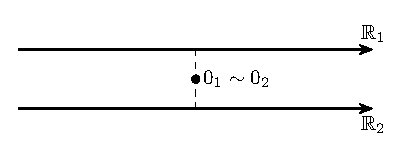
\includegraphics{images/c2.1.pdf}
        \caption{Пример нехаусдорфова пространства}
        \label{fig:c2.1}
    \end{figure}
\end{example}
% конец второй лекции